\section{Realización numérica}

\subsection{Aproximación lineal de una función}
\begin{frame}
\frametitle{\subsecname}

\begin{minipage}{0.45\paperwidth}
	Del diagrama, tenemos \[ \frac{f\left(x+h\right)-f\left(x\right)}{h}\approx f^{\prime}\left(x\right)\quad\text{para }h\text{ pequeño}. \] Reordenando la ecuación resulta \[ f\left(x+h\right)\approx f\left(x\right)+hf^{\prime}\left(x\right). \] Esto se muestra en el diagrama. La recta $\ell$ es tangente a $y=f\left(x\right)$	en el punto de coordenadas $\left(x,f\left(x\right)\right)$.
\end{minipage}
\hfill
\begin{minipage}{0.45\paperwidth}
	\begin{figure}
		\centering
		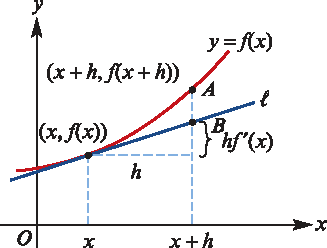
\includegraphics[width=0.4\paperwidth]{euler1}
		\caption{La recta $\ell$ es una aproximación lineal en $B$ de $y=f\left(x\right)$.}
	\end{figure}
\end{minipage}
\vfill
\begin{remark}
	Esto nos da una aproximación a la curva $y=f\left(x\right)$ en que la coordenada $y$ de $B$ es una aproximación a la coordenada $y$ de $A$ en la gráfica de $y=f\left(x\right)$.
\end{remark}
\end{frame}

\subsection{Problema de valor inicial}

\begin{frame}
	\frametitle{\subsecname}
	\begin{minipage}{0.45\paperwidth}
		Considere el problema de valor inicial \[ \frac{\mathrm{d}y}{\mathrm{d}x}=g\left(x\right)\quad\text{con}\quad y\left(x_{0}\right)=0. \] Entonces, $x_{1}=x_{0}+h$ e $y_{1}=y_{0}+hg\left(x_{0}\right)$.
	\end{minipage}
	\hfill
	\begin{minipage}{0.45\paperwidth}
		\begin{figure}
			\centering
			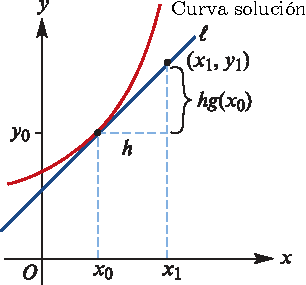
\includegraphics[width=0.4\paperwidth]{euler2}
			\caption{La diferencia en las ordenadas es $y_{1}-y_{0}=hg\left(x_{0}\right)$.}
		\end{figure}
	\end{minipage}
\end{frame}

\subsection{Método de Euler}

\begin{frame}
	\frametitle{\subsecname}
	\begin{minipage}{0.45\paperwidth}
		El proceso es ahora aplicado repetidamente para aproximar el valor de la función en $x_{2},x_{3},\ldots$.

		\

		El resultado es:
		\begin{align*}
		x_{2}&=x_{1}+h\quad\text{e}\quad y_{2}=y_{1}+hg\left(x_{1}\right),\\
		x_{3}&=x_{2}+h\quad\text{e}\quad y_{3}=y_{2}+hg\left(x_{2}\right),
		\end{align*}
		y así sucesivamente.

		\

		El punto $\left(x_{n},y_{n}\right)$ es encontrado en el $n$--ésimo\linebreak paso del proceso iterativo.

		\

		Este proceso iterativo se puede resumir de la \linebreak siguiente manera.
	\end{minipage}
	\hfill
	\begin{minipage}{0.45\paperwidth}
		\begin{figure}
			\centering
			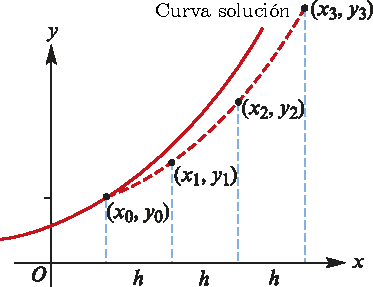
\includegraphics[width=0.4\paperwidth]{euler3}
			\caption{Los puntos $\left(x_{0},y_{0}\right)$, $\left(x_{1},y_{1}\right)$, $\left(x_{2},y_{2}\right)$ y $\left(x_{3},y_{3}\right)$ se aproximan a la curva solución.}
		\end{figure}
	\end{minipage}
\end{frame}

\begin{frame}
\frametitle{\subsecname}

\begin{minipage}{0.45\paperwidth}
	\begin{theorem}[Método de Euler]
			Si $\frac{\mathrm{d}y}{\mathrm{d}x}=g\left(x\right)$ con $x_{0}=a$ e $y_{0}=b$, entonces \[ x_{n+1}=x_{n}+h\quad\text{e}\quad y_{n+1}=hg\left(x_{n}\right). \]
	\end{theorem}
\end{minipage}
\hfill
\begin{minipage}{0.45\paperwidth}
	\begin{figure}
		\centering
		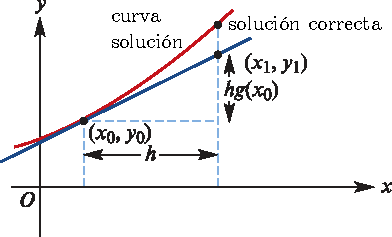
\includegraphics[width=0.4\paperwidth]{euler4}
		\caption{.}
	\end{figure}
\end{minipage}
\end{frame}

%\subsubsection{Método de Runge-Kutta}

\begin{frame}[fragile]
\frametitle{\subsecname}

\begin{pylabcode}[plotsession]
rc('text', usetex=True)
rc('font', **{'family':'serif', 'serif':['Times']})
rc('legend', fontsize=10.0)
def f(t): return (t**3)/3-t**2
t1 = arange(0.0, 4.0, 0.01)
x0, y0, xf, n = 0, 1, 5, 201
deltax = (xf-x0)/(n-1)
x = linspace(x0, xf, n)
y = zeros([n])
y[0] = 0
for i in range(1, n): y[i] = deltax*( x[i - 1]*x[i - 1] - 2*x[i-1] )
plot(x, y, 'b--',t1, f(t1), 'r--')
xlabel("Valores de x")
ylabel("Valores de y")
title("Solución aproximada con el método de Euler vs la solución exacta")
savefig('images/eulersol.pdf', bbox_inches='tight')
\end{pylabcode}

\begin{minipage}{0.45\paperwidth}
\begin{example}
	Considere el problema de valor inicial \[ \frac{\mathrm{d}y}{\mathrm{d}x}=-y+\operatorname{sen}\left(x\right),\quad y\left(0\right)=1. \]
\end{example}
\vfill
\begin{figure}[H]
	\centering
	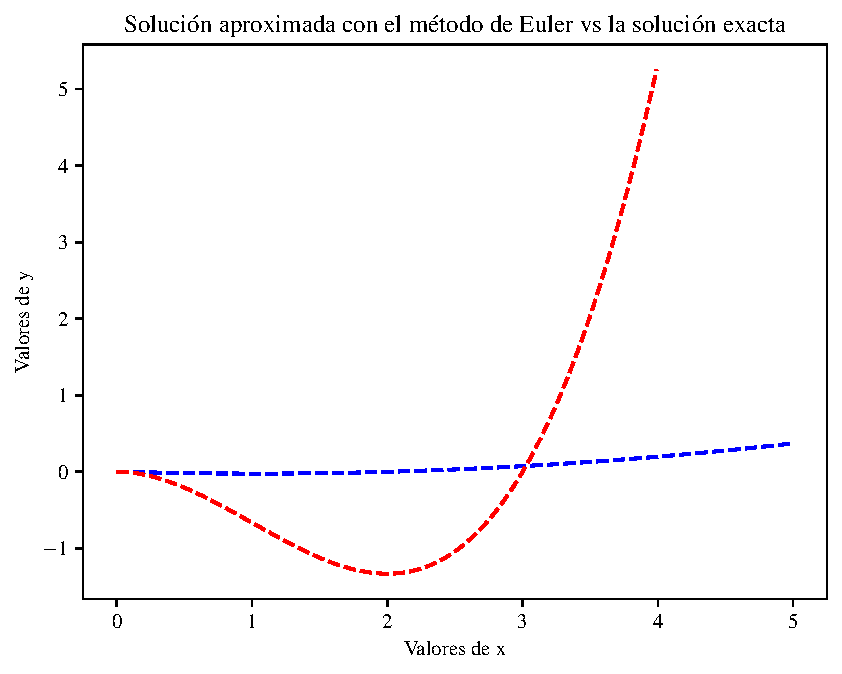
\includegraphics[width=0.4\paperwidth]{eulersol}
	\caption{\label{fig:matlpotlib}Solución exacta vs solución de Euler}
\end{figure}
\end{minipage}
\hfill
\begin{minipage}{0.45\paperwidth}
		\begin{listing}[H]
		\inputminted{python}{./code/euler_01.py}
		\caption{Programa \texttt{euler.py}}
	\end{listing}
\end{minipage}
\end{frame}